\documentclass[10pt,a4paper]{article}
\usepackage[margin=19mm]{geometry}
\usepackage[T1]{fontenc}
\usepackage{lmodern,graphicx,booktabs,array,amsmath,amssymb,hyperref,float,tikz,xcolor,caption}
\usetikzlibrary{arrows.meta,positioning,shapes.geometric}
\hypersetup{colorlinks=true,urlcolor=blue,linkcolor=blue}
\setlength{\parindent}{0pt}\setlength{\parskip}{5pt}
\graphicspath{{figures/}{../building-block/figures/}{../dc-link/figures/}{../../simulation/sharing/}}
\newcommand{\uF}{\ensuremath{\mu}F}
\newcolumntype{L}[1]{>{\raggedright\arraybackslash}p{#1}}
%% generated by scripts/bb_losses.py
\newcommand{\Prated}{2.65}
\newcommand{\Pbudget}{13.3}
\newcommand{\Ipk}{141}
\newcommand{\CreqBlock}{78}
\newcommand{\CreqTotal}{233}
\newcommand{\CreqAlone}{236}
\newcommand{\CeffBlock}{77}
\newcommand{\dVshared}{3.0}
\newcommand{\dValone}{9.1}
\newcommand{\IlegHFworst}{50}
\newcommand{\IlegHFrated}{29}
\newcommand{\IthreeHF}{65}
\newcommand{\PcondTyp}{5.55}
\newcommand{\PcondMax}{7.40}
\newcommand{\PcondCold}{3.75}
\newcommand{\Pdead}{0.20}
\newcommand{\Pgate}{0.078}
\newcommand{\Pcap}{0.39}
\newcommand{\PcuHf}{1.07}
\newcommand{\PcuTot}{4.37}
\newcommand{\PcuHfLowM}{2.5}
\newcommand{\PcapOld}{0.08}
\newcommand{\Pcu}{3.30}
\newcommand{\Psw}{1.91}
\newcommand{\Ptot}{12.49}
\newcommand{\PcuOneOz}{4.67}
\newcommand{\PcuAC}{1.46}
\newcommand{\PcuDCP}{0.90}
\newcommand{\PcuDCN}{0.94}
\newcommand{\RacPath}{0.146}
\newcommand{\RdcpPath}{0.216}
\newcommand{\RdcnPath}{0.226}
\newcommand{\RdcpPathOneOz}{0.353}
\newcommand{\RdcnPathOneOz}{0.420}
\newcommand{\IdcpRms}{65}
\newcommand{\LloopTwoOz}{0.376}
\newcommand{\Eta}{99.53}
\newcommand{\EtaWorst}{99.46}
\newcommand{\PtotWorst}{14.34}
\newcommand{\Eavg}{38.1}
\newcommand{\Fmax}{60}
\newcommand{\Pdev}{1.91}
\newcommand{\Tj}{64}
\newcommand{\Idev}{35.4}
\newcommand{\LloopCu}{0.312}
\newcommand{\LloopEsl}{0.374}
\newcommand{\LloopLocalEsl}{0.399}
\newcommand{\LgateOne}{1.70}
\newcommand{\LgateBoth}{2.21}
\newcommand{\RhiPath}{0.369}
\newcommand{\RloPath}{0.413}
\newcommand{\CbootSel}{1}
\newcommand{\CbootMin}{680}
\newcommand{\BootDroop}{68}
\newcommand{\RgOn}{2}
\newcommand{\RgOff}{0}
\newcommand{\VdsH}{83.1}
\newcommand{\VdsL}{85.1}
\newcommand{\VgsBump}{0.98}
\newcommand{\VgsMin}{-1.29}
\newcommand{\EonPk}{47.4}
\newcommand{\EoffPk}{8.4}
\newcommand{\DvdtOn}{12}
\newcommand{\DvdtOff}{32}

% generated by scripts/design_report.py
\newcommand{\TotNone}{16.2}
\newcommand{\EtaNone}{99.39}
\newcommand{\PdevNone}{6.4}
\newcommand{\CondNone}{11.1}
\newcommand{\SwNone}{1.4}
\newcommand{\TotNtwo}{11.1}
\newcommand{\EtaNtwo}{99.58}
\newcommand{\PdevNtwo}{1.9}
\newcommand{\CondNtwo}{5.5}
\newcommand{\SwNtwo}{1.9}
\newcommand{\TotNthree}{9.8}
\newcommand{\EtaNthree}{99.63}
\newcommand{\PdevNthree}{1.0}
\newcommand{\CondNthree}{3.7}
\newcommand{\SwNthree}{2.4}
\newcommand{\TotNfour}{9.4}
\newcommand{\EtaNfour}{99.65}
\newcommand{\PdevNfour}{0.7}
\newcommand{\CondNfour}{2.8}
\newcommand{\SwNfour}{2.9}
\newcommand{\FoptSingle}{39}
\newcommand{\FoptInter}{26}
\newcommand{\LossOptSingle}{11.7}
\newcommand{\RipRmsFifty}{4.4}
\newcommand{\RipRmsTwenty}{11.1}
\newcommand{\Lph}{15}
\newcommand{\Rac}{15}
\newcommand{\Kfe}{0.6}
\newcommand{\Area}{8.5}
\newcommand{\PdArea}{0.31}
\newcommand{\PdVol}{764}
\newcommand{\Pmax}{3.05}
\newcommand{\PdAreaMax}{0.36}

% generated by scripts/design_report_v2.py
\newcommand{\DpuMax}{3.75}
\newcommand{\DpuTyp}{2.81}
\newcommand{\KanNHmm}{1.40}
\newcommand{\KqNHmm}{1.60}
\newcommand{\LfixNH}{0.18}
\newcommand{\LanCell}{0.14}
\newcommand{\DidtCell}{27}
\newcommand{\LloopMaxNine}{0.56}
\newcommand{\RoffMaxMin}{1.9}
\newcommand{\RoffMaxTyp}{2.7}
\newcommand{\RonTot}{3.0}
\newcommand{\RoffTot}{0.8}
\newcommand{\RdampMin}{0.97}
\newcommand{\ZetaOn}{2.2}
\newcommand{\ZetaOff}{0.58}
\newcommand{\VbumpMiller}{0.33}
\newcommand{\Fcross}{98}
\newcommand{\Icap}{2.5}
\newcommand{\NcapHundred}{12}
\newcommand{\AreaHundred}{6.2}
\newcommand{\Afixed}{4.2}
\newcommand{\RhoFifty}{0.31}
\newcommand{\RhoHundred}{0.42}
\newcommand{\EtaHundred}{99.45}
\newcommand{\RhoMaxCi}{0.42}
\newcommand{\RthHsFifty}{7.3}
\newcommand{\RthHsFiftyCool}{9.9}
\newcommand{\Rtim}{1.9}
\newcommand{\UtilBump}{89}
\newcommand{\UtilRipple}{100}
\newcommand{\UtilVds}{67}
\newcommand{\UtilWorst}{108}
\newcommand{\Tone}{10.7}
\newcommand{\CdptTwo}{575}
\newcommand{\CdptFive}{233}
\newcommand{\Fring}{258}
\newcommand{\Trise}{2.4}
\newcommand{\LreqTwentyFive}{53}
\newcommand{\LreqFifty}{27}
\newcommand{\LreqHundred}{13}


\title{Design Report\\[3pt]\large GaN phase-leg building block for stacked polyphase bridge traction drives\\ 75\,V, 100\,A$_\mathrm{rms}$, 2\,$\times$\,EPC2361 per switch}
\author{PCB-Design project, KTH}
\date{7 October 2026 --- design study, simulation-based (no hardware yet)}

\begin{document}
\maketitle

\begin{abstract}
This report documents the step-by-step design of a phase-leg building block for a stacked polyphase bridge (SPB) traction drive.
Each step states its objective, the options considered, the decision, and the evidence from analysis, Ansys Q3D extraction and LTspice simulation.
The design aims at high efficiency (low switching and conduction loss), high power density, and a high switching frequency (smaller DC link and lower current ripple delivered to the machine), while keeping the parasitics small and symmetric so that two paralleled GaN devices share current.
Result: \Prated\,kW per leg on a 30\,$\times$\,28\,mm four-layer board (\PdArea\,kW/cm$^2$), 0.37\,nH commutation-loop inductance per cell (Q3D, copper + MLCC ESL), $<$0.1\,\% left/right asymmetry, R$_\mathrm{g,on}$/R$_\mathrm{g,off}$\,=\,\RgOn/\RgOff\,$\Omega$, and \Eta\,\% estimated efficiency at 50\,kHz (\EtaHundred\,\% at 100\,kHz).
\end{abstract}

\begin{table}[H]\centering\small
\begin{tabular}{@{}lr@{}}\toprule
Key result & Value \\\midrule
Power per leg (M = 1, $\cos\varphi$ = 1) / maximum (M = 1.15) & \Prated\,/\,\Pmax\,kW \\
Board area, power density (board level, without cooling) & \Area\,cm$^2$, \PdArea\,kW/cm$^2$ \\
Loss at 50\,kHz / efficiency (typ.\ R$_\mathrm{DS(on)}$, 100\,$^\circ$C) & \Ptot\,W / \Eta\,\% \\
Efficiency at 100\,kHz & \EtaHundred\,\% (below target) \\
Commutation-loop inductance per cell (Q3D, incl.\ MLCC ESL) & \LloopEsl\,nH \\
Peak V$_\mathrm{DS}$ at 160\,A (13\,\% overload) & \VdsH\,V (QH), \VdsL\,V (QL) \\
Gate loop per FET; current imbalance between paralleled FETs & \LgateOne\,nH; $<$0.1\,\% \\
DC-link (effective) per leg & \CeffBlock\,\uF{} (24\,$\times$\,10\,\uF{} + 12\,$\times$\,1\,\uF) \\
\bottomrule\end{tabular}\end{table}

\section{Design objectives and flow}
\begin{table}[H]\centering\small
\begin{tabular}{@{}L{4.2cm}L{5.8cm}L{5.6cm}@{}}\toprule
Objective & Metric & Target \\\midrule
Efficiency & loss per leg at the rated point & $\geq$\,99.5\,\% ($\leq$\,\Pbudget\,W) \\
High switching frequency & $f_\mathrm{sw}$ at which the target is still met & 50\,kHz nominal (target met up to \Fmax\,kHz) \\
Winding current ripple & $\Delta i_\mathrm{pp}\approx V_\mathrm{dc}/(4Lf_\mathrm{sw})$ & requirement handed to the machine design \\
Device safety & peak $V_\mathrm{DS}$, $V_\mathrm{GS}$ & $\leq$\,90\,V; $-4\dots+6$\,V \\
Paralleling & dynamic and static current imbalance & as small as the layout allows \\
Power density & board area per kW & as small as cooling and probing allow \\
\bottomrule\end{tabular}\end{table}

\begin{figure}[H]\centering
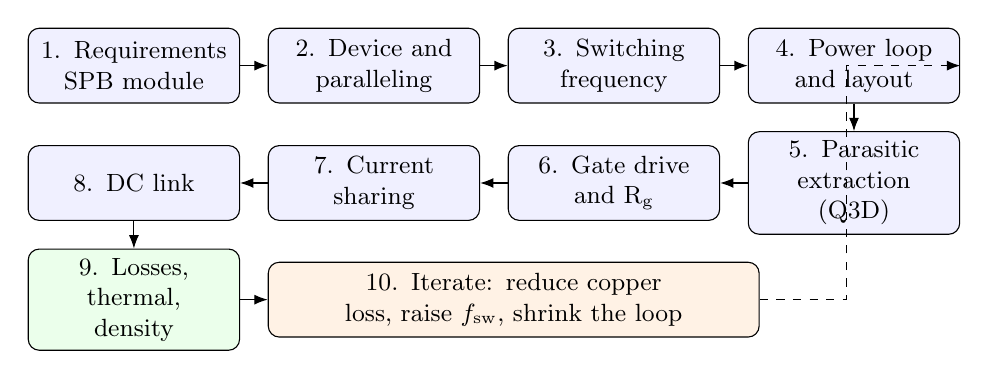
\begin{tikzpicture}[node distance=0.35cm and 0.35cm, font=\small,
  st/.style={draw,rounded corners,fill=blue!6,minimum height=0.95cm,text width=2.45cm,align=center},>=Latex]
\node[st] (a) {1. Requirements\\SPB module};
\node[st,right=of a] (b) {2. Device and\\paralleling};
\node[st,right=of b] (c) {3. Switching\\frequency};
\node[st,right=of c] (d) {4. Power loop\\and layout};
\node[st,below=of d] (e) {5. Parasitic\\extraction (Q3D)};
\node[st,left=of e] (f) {6. Gate drive\\and R$_\mathrm{g}$};
\node[st,left=of f] (g) {7. Current\\sharing};
\node[st,left=of g] (h) {8. DC link};
\node[st,below=of h,fill=green!8] (i) {9. Losses, thermal,\\density};
\node[st,right=of i,fill=orange!10,text width=6.0cm] (j) {10. Iterate: reduce copper loss, raise $f_\mathrm{sw}$, shrink the loop};
\draw[->] (a)--(b); \draw[->] (b)--(c); \draw[->] (c)--(d); \draw[->] (d)--(e); \draw[->] (e)--(f); \draw[->] (f)--(g); \draw[->] (g)--(h); \draw[->] (h)--(i); \draw[->] (i)--(j);
\draw[->,dashed] (j.east) -| ++(1.1,1.4) |- (d.east);
\end{tikzpicture}
\caption{Design flow. Steps 4--7 are coupled through the parasitics: the layout sets the loop and gate inductances, which set the gate resistors, which set the switching loss and the overshoot.}
\end{figure}

\section{Step 1 --- Requirements from the SPB system}
In an SPB the DC bus is split into $N$ series-stacked modules, each driving its own phase group of a multiphase machine and seeing only $V_\mathrm{dc}/N$. With 100\,V GaN devices the module bus is set to 75\,V ($N\approx11$ for 800\,V), leaving a 15\,V design margin for overshoot (90\,V) and 25\,V to the rating. Phase current 100\,A$_\mathrm{rms}$ (\Ipk\,A peak); rated power per leg \Prated\,kW; efficiency target 99.5\,\%.
The SPB motivates the design objectives: (i) a cheap, fast, low-voltage device class becomes usable for 800\,V traction; (ii) the voltage step per module is only 75\,V, so dv/dt stress on the winding is much smaller than with a full-bus SiC inverter; (iii) one building block is repeated $N$ times, so its density and efficiency multiply.

\section{Step 2 --- Device and number in parallel}
\textbf{Device.} EPC2361: 100\,V, 0.75/1.0\,m$\Omega$, $Q_\mathrm{G}$\,=\,28\,nC, $Q_\mathrm{rr}$\,=\,0, 3\,$\times$\,5\,mm, top-side cooling (R$_\mathrm{thJC}$\,=\,0.2\,K/W). Its figure of merit allows fast, low-loss switching at 75\,V; the absence of reverse recovery removes the dominant turn-on loss of silicon.

\textbf{How many in parallel.} Conduction loss falls as $1/n$; the current-independent part of the switching energy (output charge) rises with $n$; area, loop length and sharing risk grow with $n$.
\begin{figure}[H]\centering
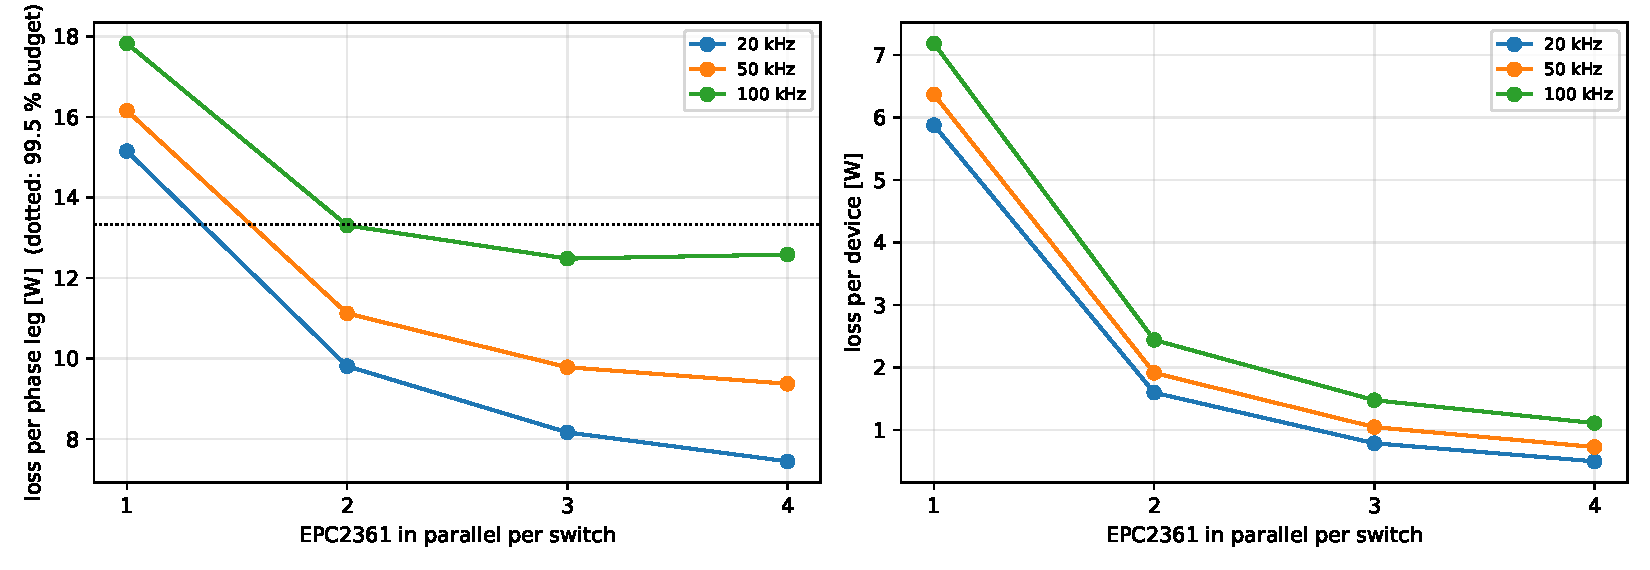
\includegraphics[width=0.92\textwidth]{n_parallel.pdf}
\caption{Loss per leg and per device versus the number of EPC2361 per switch (switching energy scaled from the $n$\,=\,2 LTspice fit; copper loss kept constant).}
\end{figure}
\begin{table}[H]\centering\small
\begin{tabular}{@{}lcccc@{}}\toprule
At 50\,kHz & $n$ = 1 & $n$ = 2 & $n$ = 3 & $n$ = 4 \\\midrule
Conduction [W] & \CondNone & \CondNtwo & \CondNthree & \CondNfour \\
Switching [W] & \SwNone & \SwNtwo & \SwNthree & \SwNfour \\
Total incl.\ copper [W] / efficiency [\%] & \TotNone\,/\,\EtaNone & \TotNtwo\,/\,\EtaNtwo & \TotNthree\,/\,\EtaNthree & \TotNfour\,/\,\EtaNfour \\
Loss per device [W] & \PdevNone & \PdevNtwo & \PdevNthree & \PdevNfour \\
\bottomrule\end{tabular}\end{table}
\textbf{Decision: $n$\,=\,2.} One device misses the target and dissipates 6.4\,W per device. Two meet it with margin. Three or four gain only 1.3--1.7\,W while increasing area, loop length and sharing risk.\textit{Note: the scaling assumes the same layout quality for every $n$; in reality $n\geq3$ lengthens the loop.}

\section{Step 3 --- Switching frequency}
A higher $f_\mathrm{sw}$ shrinks the DC-link capacitance (Step 8) and the current ripple delivered to the machine ($\propto1/f_\mathrm{sw}$), but raises the inverter switching loss linearly, by about 0.44\,W per 10\,kHz for this block (Step 9).

\textbf{Winding ripple requirement.} The machine is not yet defined, so machine-side PWM losses are not evaluated here. The inverter side can, however, state what it requires: the peak-to-peak ripple of a phase is at most $\Delta i_\mathrm{pp}\approx V_\mathrm{dc}/(4L f_\mathrm{sw})$, where $L$ is the inductance seen by the ripple. For $\Delta i_\mathrm{pp}\leq10$\,\% of the 141\,A peak this means $L\geq$\,\LreqTwentyFive, \LreqFifty{} and \LreqHundred\,\textmu H at 25, 50 and 100\,kHz, a requirement to be handed to the machine design.

\textbf{Decision: 50\,kHz nominal.} 50\,kHz halves the DC-link capacitance and the ripple compared with 25\,kHz and still meets the efficiency target (\Eta\,\%). With typical devices the target is met up to \Fmax\,kHz; 100\,kHz (\EtaHundred\,\%) needs the copper improvements of Step 10. The final value is fixed once the machine is selected.

\section{Step 4 --- Power loop and layout: minimising the parasitics}
\textbf{Constraint.} $\Delta V=L_\mathrm{loop}\,di_\mathrm{cell}/dt\leq15$\,V. With about 40\,A/ns through one cell (FET pair) this gives $L_\mathrm{loop}\lesssim0.37$\,nH.

\textbf{Measures, each quantified with Q3D:}
\begin{enumerate}\itemsep1pt
\item \emph{Vertical (inner-layer) loop.} Forward current on L1, return on L2 directly underneath: flux cancellation. Loop inductance scales with the L1--L2 dielectric: 0.075/0.1/0.2\,mm gives 0.30/0.34/0.50\,nH (copper). Chosen 0.1\,mm (two-ply prepreg, 0.9\,kV/mm at 90\,V).
\item \emph{Commutation capacitors at the high-side drain.} 6\,$\times$\,1\,\uF{} 0805 per cell in parallel; their ESL adds only about 0.08\,nH. Placement variants (single cell, with ESL): bank at QH 0.39\,nH, bank between QH and QL 0.38\,nH (but switch-node plane on L2), two banks with a close L2/L3 pair 0.33\,nH.
\item \emph{Two mirrored cells.} Each FET pair has its own commutation loop and carries half of the load current, so its $di/dt$ is halved; the loop inductance itself is not reduced. Mirror symmetry makes left and right identical ($<$0.1\,\%).
\item \emph{Dense via rows, no plane cuts under the cells, short wide copper; DC+ and AC brought in on inner planes so that L1 stays compact.}
\end{enumerate}

\begin{figure}[H]\centering
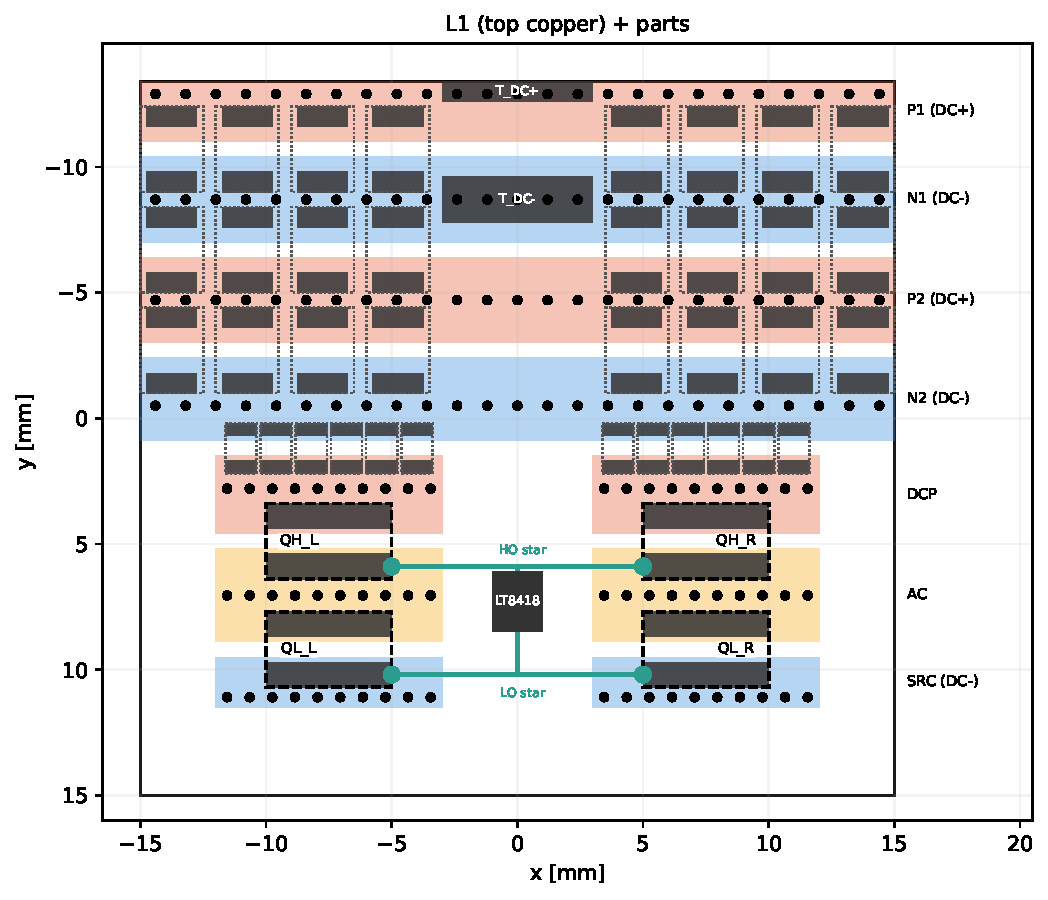
\includegraphics[width=0.62\textwidth]{layout_top.pdf}\hfill
\begin{minipage}[b]{0.36\textwidth}
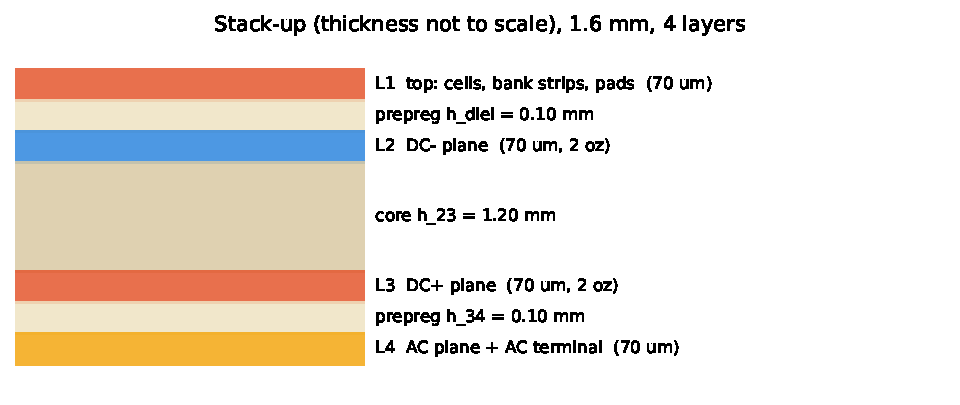
\includegraphics[width=\textwidth]{layout_stackup.pdf}\\[4pt]
\small 30\,$\times$\,28\,mm, 4 layers, 2\,oz. L2 DC$-$, L3 DC+, L4 AC. Driver on the symmetry line, terminals on the centre line.
\end{minipage}
\caption{Building-block layout (generated from the same geometry as the Q3D model).}
\end{figure}

\section{Step 5 --- Parasitic extraction}
Q3D models only the copper; every component is a gap with source and sink terminals on its pads. The resulting partial $R$/$L$ matrix (21 terminals) is exported to LTspice with coupling coefficients, so the circuit simulation sees the real layout.
\begin{table}[H]\centering\small
\begin{tabular}{@{}lr@{}}\toprule
Commutation loop per cell (copper / with MLCC ESL) & \LloopCu\,/\,\LloopEsl\,nH \\
Gate loop per FET (one / both driven) & \LgateOne\,/\,\LgateBoth\,nH \\
DC resistance terminal-to-FETs, DC+ / DC$-$ / AC (2\,oz) & \RdcpPath\,/\,\RdcnPath\,/\,\RacPath\,m$\Omega$ \\
\bottomrule\end{tabular}\end{table}
\textbf{Loop inductance and paralleling.} Each FET sees its own cell loop of 0.374\,nH; paralleling does not reduce it. Q3D excites both cells simultaneously (1\,A each), so this value already contains the mutual coupling through the shared bank and planes. Paralleling reduces the current each loop commutates: each cell carries half the load current, so its $di/dt$ and therefore its overshoot are lower. The value excludes the EPC2361 package inductance and post-routing details, so the real loop will be somewhat higher; the DPT ringing frequency will give the measured value.

The extraction also revealed a non-obvious loss: the DC planes carry about 65\,A$_\mathrm{rms}$ of switching-averaged current over 15--20\,mm, so the PCB copper costs \PcuOneOz\,W with 1\,oz inner layers and \Pcu\,W with 2\,oz (adopted) at the load-current frequency.

\textbf{Switching-harmonic copper loss.} A Q3D frequency sweep (1\,kHz--100\,MHz) shows that the copper resistance is already about 1.5$\times$ its DC value at 50\,kHz and 3$\times$ at 500\,kHz, because the current crowds onto the facing surfaces and the lowest-inductance paths of the planes. Solving the board network (Q3D $R(f)$, $L(f)$, MLCC groups, DC-supply impedance, switched FET currents for SVM) at every harmonic gives \PcuHf\,W of copper loss at the switching harmonics on top of the \Pcu\,W from the load current, up to \PcuHfLowM\,W at low modulation index where the ripple current is largest. Most of the ripple current comes from the 1210 bank above the cells and crosses the planes; the same network gives \Pcap\,W of MLCC ESR loss.

\section{Step 6 --- Gate drive and gate resistors}
\textbf{Driver requirements} (from the design): rating $\geq$\,95\,V (prefer $\geq$\,110\,V); bootstrap clamp (the switch node goes 2--3\,V negative in dead time, which would overcharge the bootstrap above the 6\,V GaN limit); source $\geq$\,2--4\,A, sink $\geq$\,4\,A with split outputs; dv/dt immunity $\geq$\,100\,V/ns; delay matching of a few ns.
\begin{table}[H]\centering\small
\begin{tabular}{@{}L{3.3cm}lL{2.9cm}L{5.0cm}L{1.9cm}@{}}\toprule
Driver & Rating & Source / sink & Notes & Verdict \\\midrule
TI LMG1210 & 200\,V & 1.5 / 3\,A & too weak at 120\,A; gate bump 0.95\,V at 1\,$\Omega$ & rejected \\
uPI uP1966E (EPC90156) & 85\,V & 0.7 / 0.4\,$\Omega$ & only about 5\,V margin at 75\,V & rejected \\
ADI LT8418 & 100\,V & 4 / 8\,A (0.6/0.2\,$\Omega$) & smart bootstrap, WLCSP & baseline \\
Infineon 2EDL5014AA-U2D & 120\,V & 4 / 4\,A (0.7/0.47\,$\Omega$) & GaN bootstrap clamp, Miller clamp, 2\,$\times$\,2\,mm TSNP & strong alternative \\
\bottomrule\end{tabular}\end{table}
Both LT8418 and 2EDL5014AA give practically the same switching (at 160\,A, R$_\mathrm{g,on}$\,=\,2\,$\Omega$: 82--83\,V, bump about 1\,V; E$_\mathrm{off}$ +1.5--3\,\textmu J with the 2EDL). The 2EDL5014AA offers more voltage margin and easier assembly; its 6--9\,$\Omega$ bootstrap switch must be checked at high modulation index.

\textbf{Placement.} The driver sits on the symmetry line so that both FETs of each switch are driven through equal stars (1.7\,nH per branch), with Kelvin returns from each source pad. The common-source inductance is then only the pad and package part.

\textbf{Gate resistors.} Swept at 160\,A: R$_\mathrm{g,on}$ trades overshoot and Miller bump (lower bound) against E$_\mathrm{on}$ (upper bound). R$_\mathrm{g,off}$ hardly changes E$_\mathrm{off}$ (turn-off is load-driven) but weakens hold-off.
\begin{figure}[H]\centering
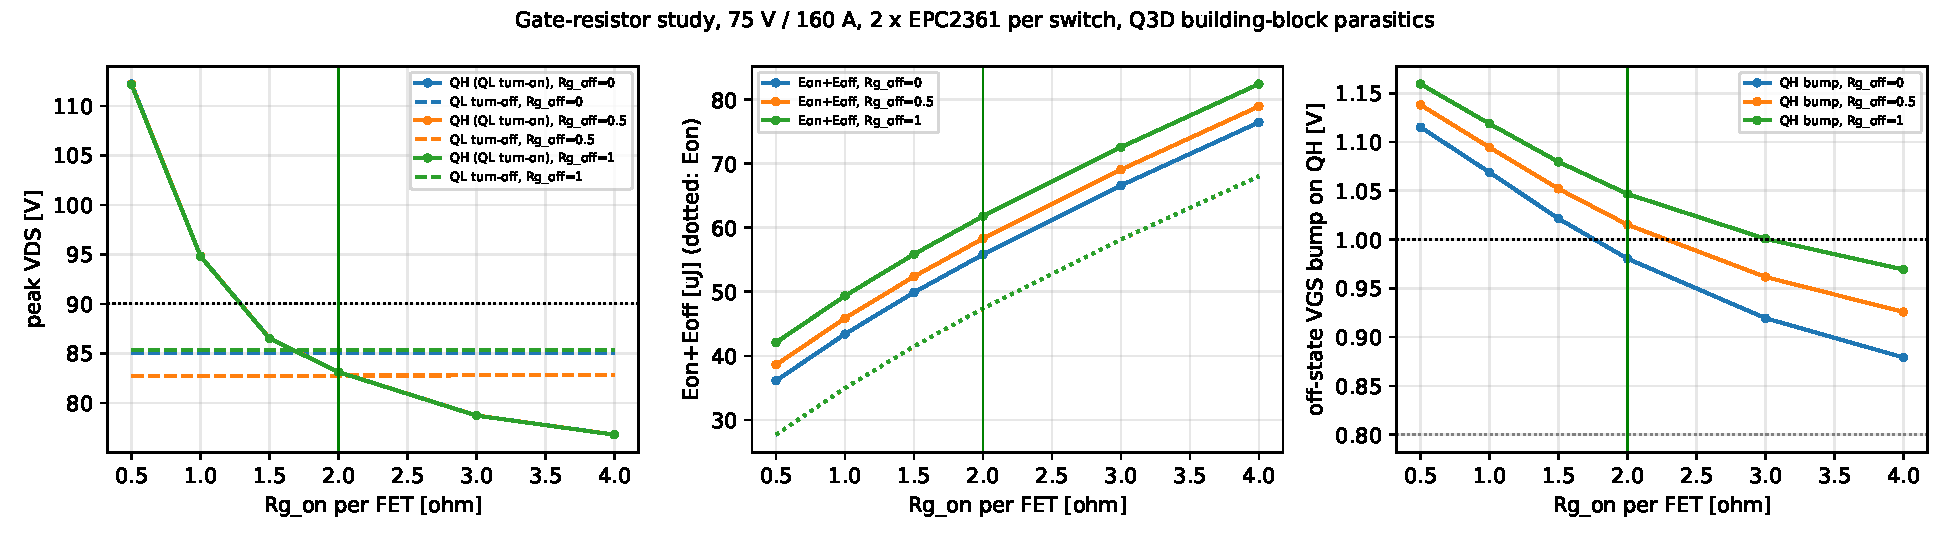
\includegraphics[width=\textwidth]{rg_study.pdf}
\caption{Gate-resistor study (LTspice with Q3D parasitics). Selected R$_\mathrm{g,on}$\,=\,2\,$\Omega$, R$_\mathrm{g,off}$\,=\,0\,$\Omega$: QH \VdsH\,V, QL \VdsL\,V, bump \VgsBump\,V. EPC's four-parallel motor-drive board uses much larger values (10\,$\Omega$ on / 2\,$\Omega$ off) because it deliberately limits dv/dt for the motor; a DPT-oriented power stage can switch faster.}
\end{figure}
Gate-loop damping: turn-on $R_\mathrm{tot}$\,=\,3.0\,$\Omega$ gives $\zeta\approx2.2$ (no V$_\mathrm{GS}$ overshoot); turn-off 0.6\,$\Omega$ gives $\zeta\approx0.44$ ($-1.3$\,V undershoot, within $-4$\,V).

\section{Step 7 --- Current sharing}
A two-device sensitivity study (one parasitic changed at a time) identified what must be symmetric:
\begin{figure}[H]\centering
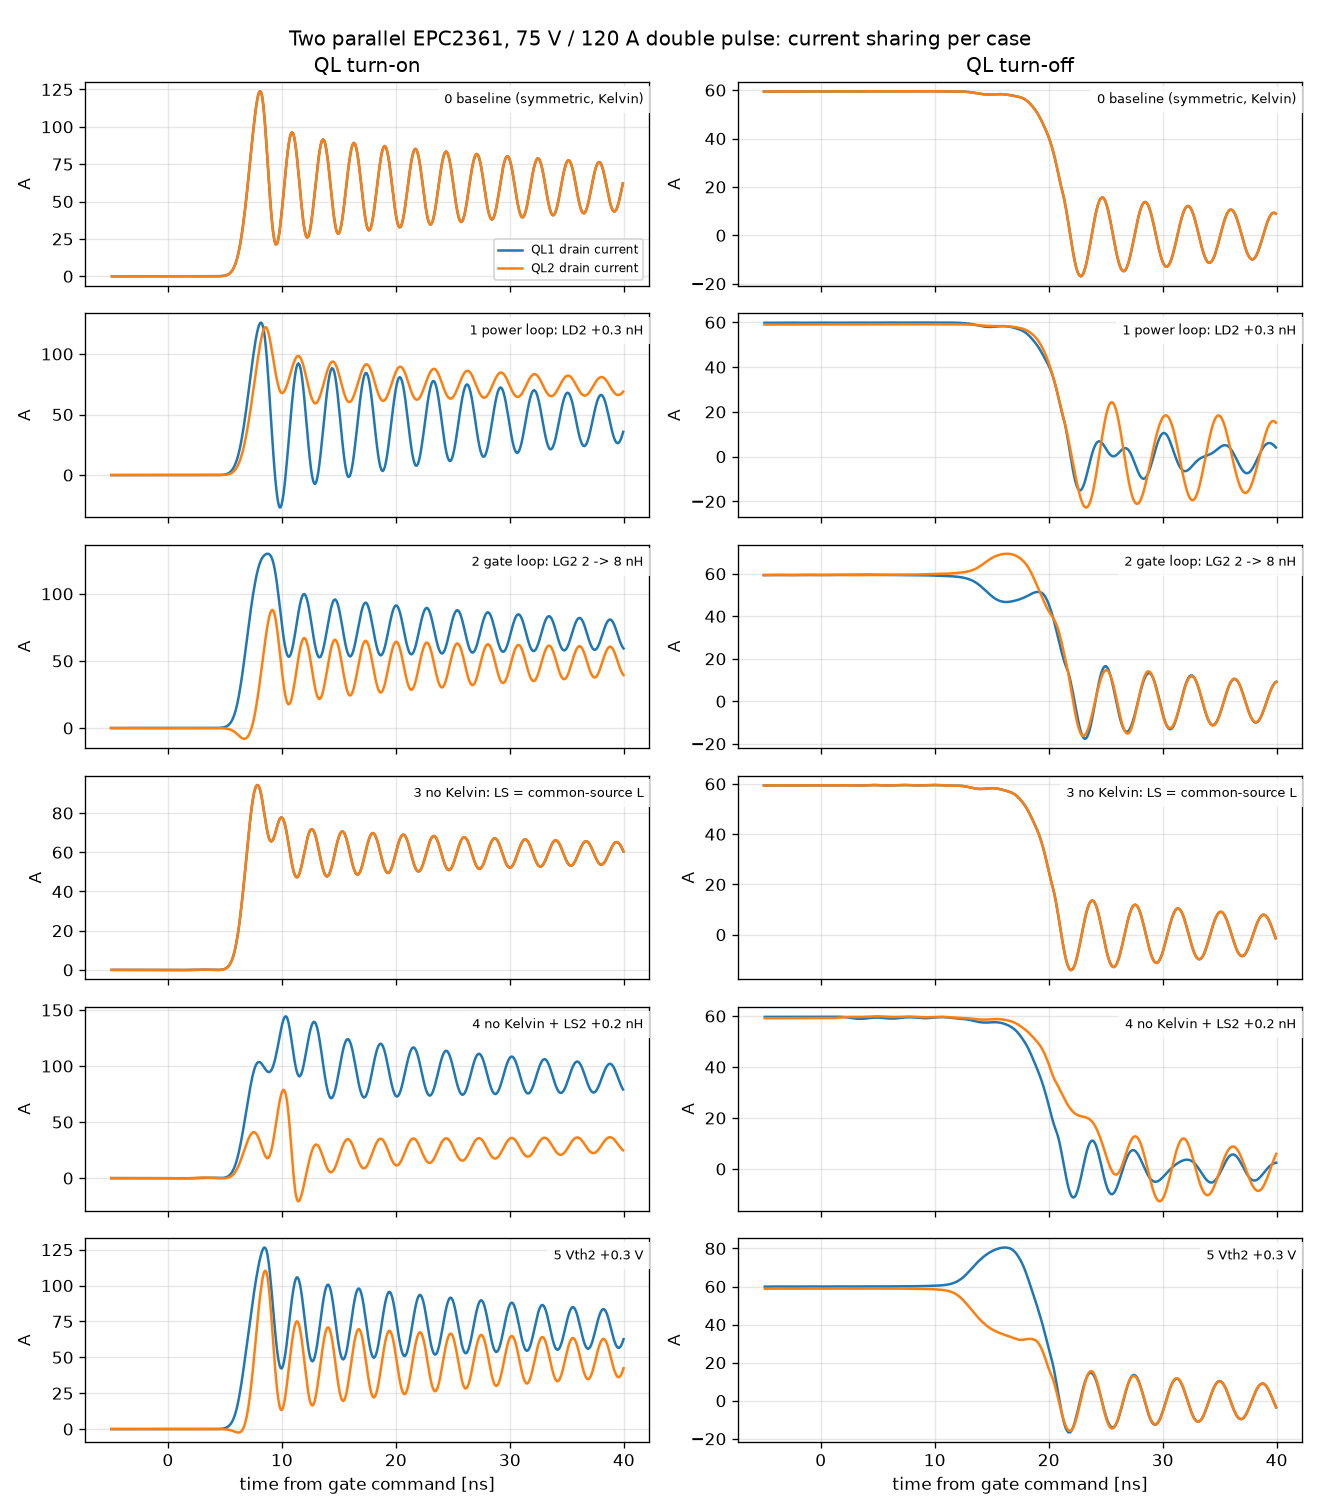
\includegraphics[width=0.72\textwidth]{Sharing_2xEPC2361.png}
\caption{Drain currents of two paralleled EPC2361 at 75\,V/120\,A for six cases: baseline; drain inductance +0.3\,nH (2\,\% imbalance, energy shift); gate loop 2$\to$8\,nH (19\,\%, 4:1 $E_\mathrm{on}$ split); no Kelvin, symmetric (slower, +47\,\% $E_\mathrm{on}$); no Kelvin with common-source imbalance (29\,\%); $V_\mathrm{th}$ +0.3\,V (7\,\%, 2:1 $E_\mathrm{off}$ split).}
\end{figure}
The gate-loop case explains the centre driver: a mismatch delays one gate by about $\Delta L_\mathrm{G}/R_\mathrm{tot}\approx2$\,ns, half of the 4\,ns transition, so one device takes most of the switching. A side-mounted driver would give 2.0 vs 7.7\,nH (Q3D); the centre driver gives equal branches. On the building block the two FETs carry 78.53 and 78.63\,A at turn-off and their waveforms overlap.
\begin{figure}[H]\centering
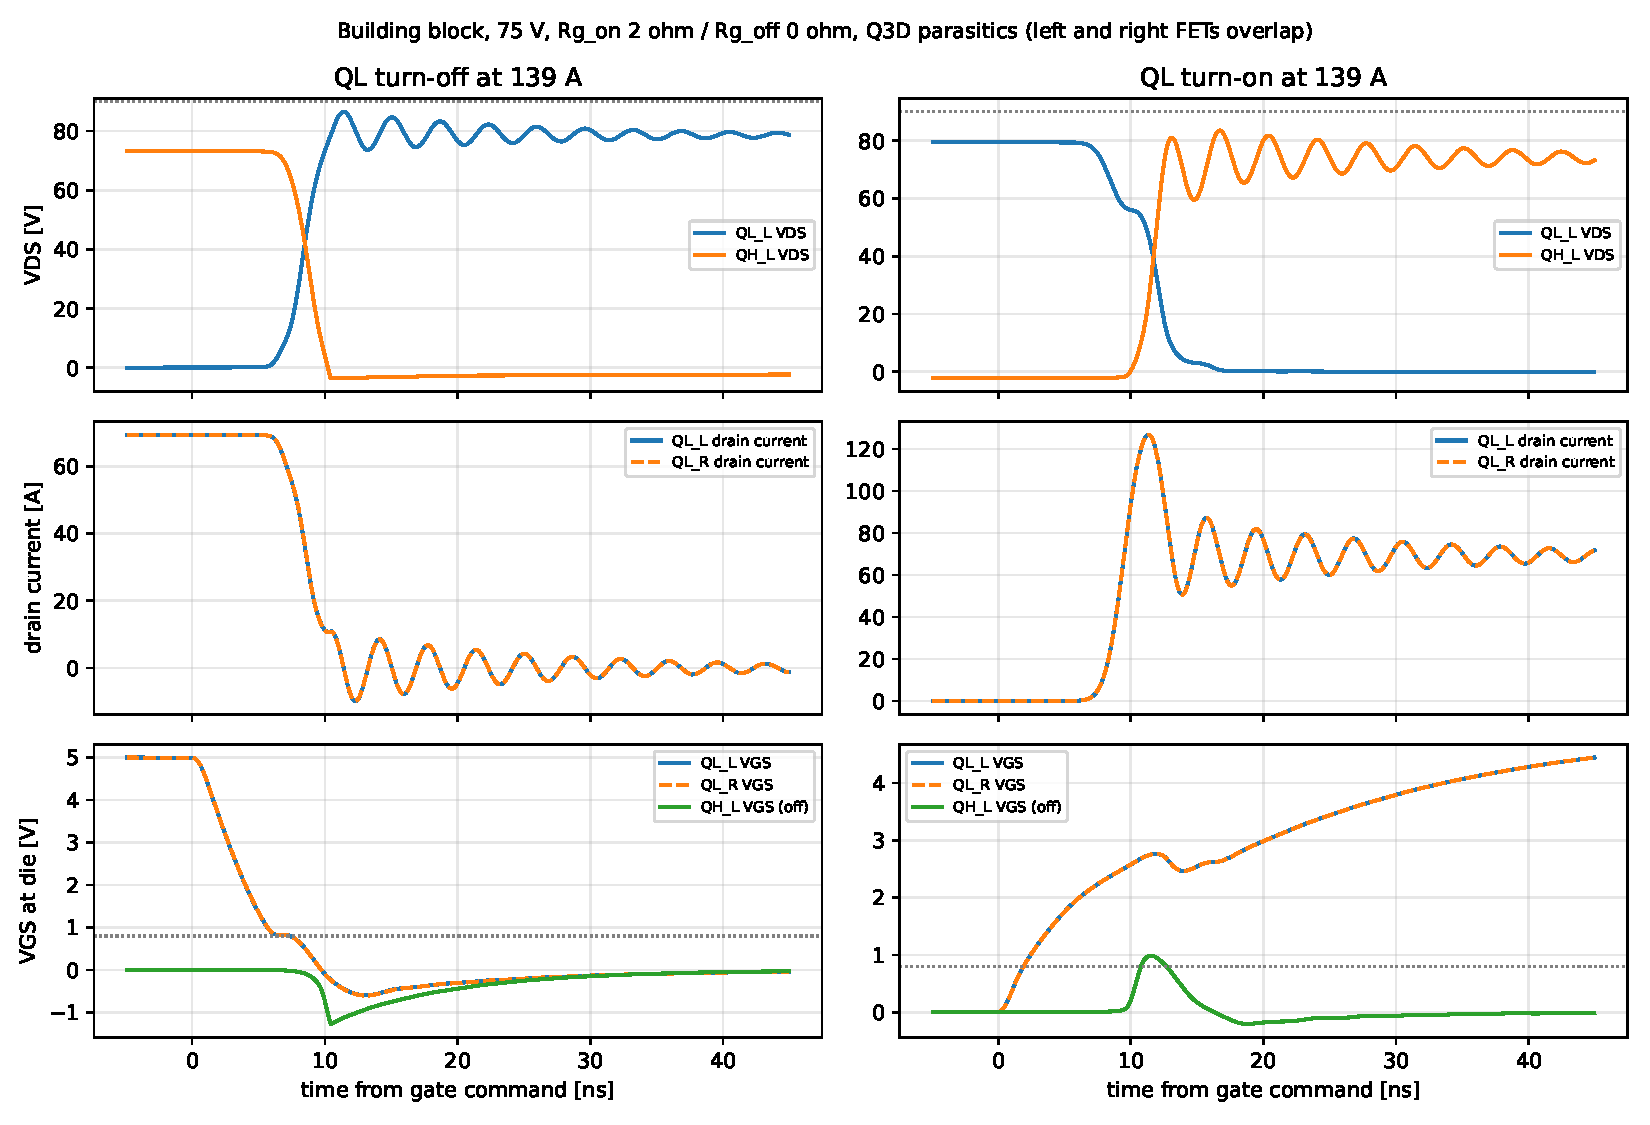
\includegraphics[width=0.82\textwidth]{waveforms_141A.pdf}
\caption{Building-block switching at the rated peak current with the selected resistors; left and right FETs overlap.}
\end{figure}

\section{Step 8 --- DC link}
Ripple current per leg: up to 50\,A$_\mathrm{rms}$ for a leg on its own, 28.8\,A at the rated point. Three legs on one bank: up to 65\,A in total. Required effective capacitance $\approx\hat I/(4f_\mathrm{sw}\Delta V_\mathrm{pp})$: 78\,\uF{} per leg for $\pm$2\,\% at 50\,kHz when three legs share a module link; half at 100\,kHz. This is the second benefit of a higher $f_\mathrm{sw}$: a smaller and denser DC link.
Selected: 24\,$\times$\,10\,\uF{} 1210 + 12\,$\times$\,1\,\uF{} 0805 (\CeffBlock\,\uF{} effective); 0.9--2.1\,A$_\mathrm{rms}$ per capacitor from a Q3D-based current-division analysis. Details: DC-link report.
\begin{figure}[H]\centering
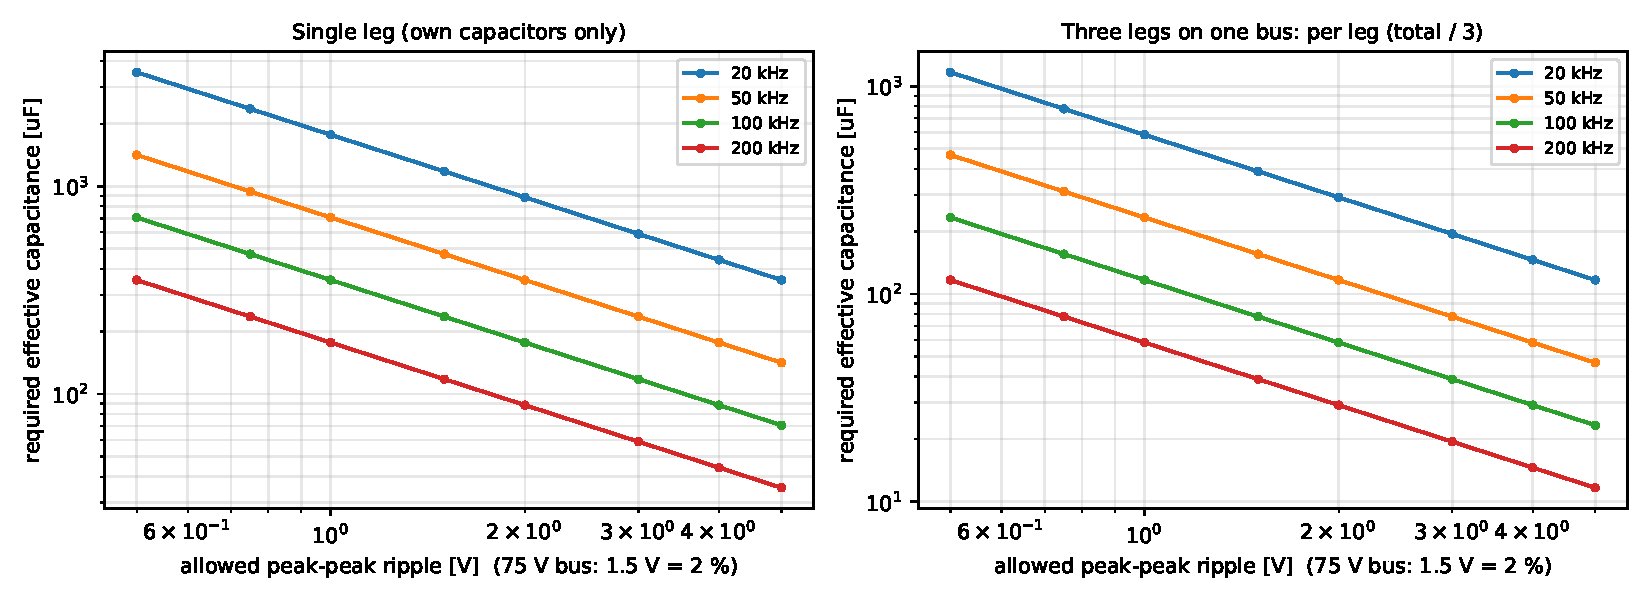
\includegraphics[width=0.85\textwidth]{creq.pdf}
\caption{Required effective capacitance versus allowed ripple for 20--200\,kHz.}
\end{figure}

\section{Step 9 --- Losses, thermal and power density}
\begin{figure}[H]\centering
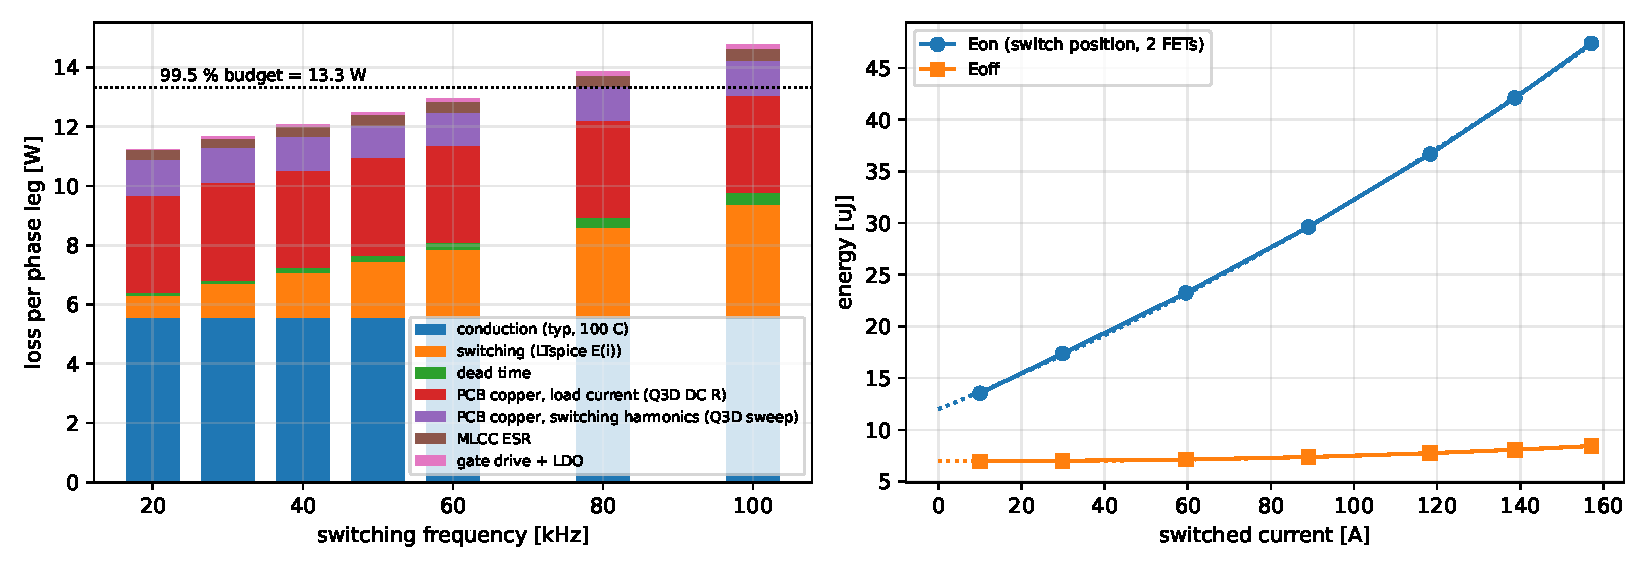
\includegraphics[width=\textwidth]{losses.pdf}
\caption{Loss per leg versus $f_\mathrm{sw}$ and switching energy versus current (LTspice with Q3D parasitics).}
\end{figure}
At 50\,kHz: conduction \PcondTyp\,W, PCB copper \Pcu\,+\,\PcuHf\,W (load current + switching harmonics), switching \Psw\,W, dead time \Pdead\,W, MLCC ESR \Pcap\,W, gate drive \Pgate\,W, total \Ptot\,W, efficiency \Eta\,\%. With maximum R$_\mathrm{DS(on)}$ the target is missed (\PtotWorst\,W, \EtaWorst\,\%). Conduction and copper are about 80\,\% of the loss, so at 50\,kHz cooling and copper matter more than switching speed. This is why the gate resistors could be chosen for safety (2\,$\Omega$) rather than minimum $E_\mathrm{on}$.

Thermal: about \Pdev\,W per device; with 0.2\,K/W junction-to-case, about 1.9\,K/W TIM and a 60\,$^\circ$C heat sink, $T_\mathrm{j}\approx$\,\Tj\,$^\circ$C.
Power density (board level): \Prated\,kW on \Area\,cm$^2$, i.e.\ \PdArea\,kW/cm$^2$ (\PdAreaMax\,kW/cm$^2$ at M\,=\,1.15), about \PdVol\,kW/L including the tallest components but excluding cooling and busbars.

\section{Step 10 --- Optimisation opportunities for the next iteration}
\begin{table}[H]\centering\small
\begin{tabular}{@{}L{5.4cm}L{5.2cm}L{5.0cm}@{}}\toprule
Measure & Expected effect & Cost / risk \\\midrule
DC busbar contacts next to each cell (not above the bank) & copper loss about $-1$ to $-1.5$\,W & mechanical design \\
AC contact directly on the L1 AC islands & AC copper loss about $-0.7$\,W & busbar/clip \\
3--4\,oz on L3/L4 only & about $-0.9$\,W & cost; keep L1/L2 thin \\
L1--L2 prepreg 0.075\,mm & loop $-12$\,\%, allows lower R$_\mathrm{g,on}$ and $E_\mathrm{on}$ & fabrication capability, insulation \\
2EDL5014AA driver & +20\,V margin, Miller clamp, easier assembly & bootstrap recharge at high M \\
Three devices per switch & $-1.3$\,W at 50\,kHz & area, loop length, sharing \\
More capacitance next to each cell & shorter ripple path, lower switching-harmonic copper loss (\PcuHf\,W today) & board area around the cells \\
Raise $f_\mathrm{sw}$ to 100\,kHz & winding ripple and DC link halved & \EtaHundred\,\%, below target unless the copper measures above are taken \\
\bottomrule\end{tabular}\end{table}
Combining the copper measures (about $-2$\,W) would bring 100\,kHz back to about 99.52\,\%, just inside the target, with half the winding ripple and half the DC-link capacitance; they also restore margin for worst-case R$_\mathrm{DS(on)}$ at 50\,kHz.

\section{Verification status and next steps}
All results are from analysis, Q3D extraction and LTspice; none are measured. The models were cross-checked against published references where possible: the loop inductance against EPC's 0.35--0.4\,nH optimal-layout range, the DC-link formulas against Kolar \& Round, and the component choices against EPC9186 and EPC90156. Next steps:
\begin{enumerate}\itemsep0pt
\item Double-pulse board: overshoot vs R$_\mathrm{g}$, $E_\mathrm{on}$/$E_\mathrm{off}$, per-device current (shunts), high-side gate bump.
\item Route the board, re-extract with Q3D, update the SPICE model.
\item When the machine is selected: check the winding-ripple requirement of Step 3 and evaluate machine-side PWM losses (separate study).
\item Confirm MLCC DC-bias data, driver availability and bootstrap behaviour at high modulation index.
\item Thermal test with the chosen TIM and heat sink.
\end{enumerate}

\section*{Decision summary}
\begin{table}[H]\centering\small
\begin{tabular}{@{}L{4cm}L{5.2cm}L{6.4cm}@{}}\toprule
Decision & Choice & Main reason \\\midrule
Module voltage & 75\,V & 100\,V GaN with 15\,V overshoot margin \\
Devices per switch & 2\,$\times$\,EPC2361 & meets 99.5\,\% with margin; knee of the loss curve \\
Switching frequency & 50\,kHz (target met up to \Fmax\,kHz) & efficiency margin; smaller DC link and ripple; final value after machine selection \\
Loop & vertical, 0.1\,mm L1--L2, caps at QH & 0.37\,nH per cell (Q3D) \\
Layout & mirrored cells, centre driver & equal gate stars and loops, $<$0.1\,\% mismatch \\
Driver & LT8418 (2EDL5014AA alternative) & 4\,A class, bootstrap protection \\
Gate resistors & 2\,$\Omega$ on / 0\,$\Omega$ off & $\leq$\,90\,V and $\leq$\,1\,V bump at 160\,A \\
Copper & 2\,oz all layers & copper loss 4.7\,$\to$\,3.3\,W \\
DC link & 24\,$\times$\,10\,\uF{} + 12\,$\times$\,1\,\uF{} & $\pm$2\,\% at 50\,kHz on a shared bus \\
\bottomrule\end{tabular}\end{table}
\end{document}
